对于一个3年期的息票来说,发行者每年付一次利息,而非到期一次性结清利息。

图\ref{fig:sys.param}给出了一个例子。
\begin{figure}[htbp]
\begin{center}
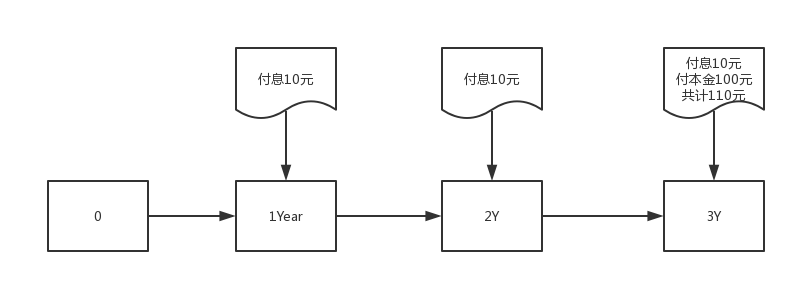
\includegraphics[width=16cm]{img//Interest_Calc.PNG}
\caption{付息日的利息计算}
\label{fig:sys.param}
\end{center}
\end{figure}

假设本金100元,年利率为$10\%$。

$PV=(v*10\%)/{(1+10\%)^1} +{(v*10\%)/(1+10\%)}^2 +{(v*(10\%+1))/(1+10\%)}^3 $

其中,第一项表示第一年付息的现值,第二项表示第二年付息的现值,第三项表示第三年付息和本金的现值。

进一步地,

$PV=(c*v)/f*∑_1^j{1/{(1+y_i/f)}^i +v/{(1+y_n/f)}^n} $

这里,我们把未来的每个现金流折现到今天。

图\ref{fig:sys.param}给出了更进一步的例子。
\begin{figure}[htbp]
\begin{center}
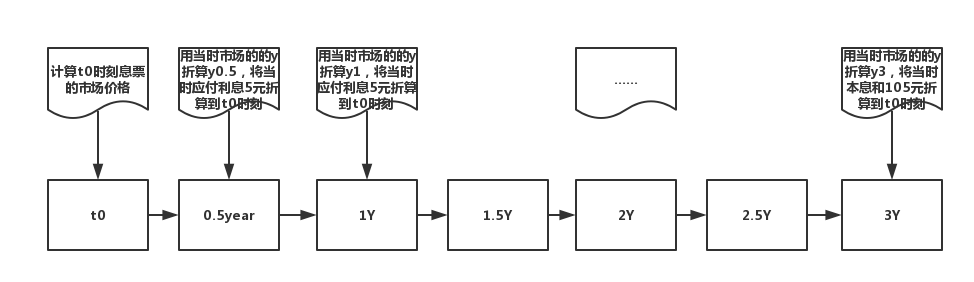
\includegraphics[width=16cm]{img//Interest_Calc_Senior.PNG}
\caption{非付息日的利息计算}
\label{fig:sys.param}
\end{center}
\end{figure}

我们将未来的现金流折现到$t_0$时刻,求得息票在$t_0$时刻的现值后,我们就可以知道应当以多少钱在市场上购入/卖出该息票。这里的$y_0.5, y_1, \cdots y_3$,指的是yield to maturity(到期收益率)。